\documentclass[11pt,aspectratio=169]{beamer}

\usetheme{Singapore}
\usecolortheme{orchid}

\usepackage[utf8]{inputenc}
\usepackage[russian]{babel}
\usepackage{amsmath}
\usepackage{amsfonts}
\usepackage{amssymb}
\usepackage{graphicx}
\usepackage{bibentry}
\usepackage{wasysym}
\usepackage[most]{tcolorbox}
\usepackage[normalem]{ulem}

\usepackage{hyperref}

\definecolor{info}{RGB}{62, 180, 137}
\definecolor{warn}{RGB}{128, 0, 0}

\author{Николай Анохин}
\title{МОБОД-2022}
\subtitle{Рекомендательные сервисы в продакшене}

\logo{
\includegraphics[width=.05\textwidth]{images/ok_logo.png}}

\AtBeginSection[]{
  \begin{frame}
  \vfill
  \centering
  \begin{beamercolorbox}[sep=8pt,center,shadow=true,rounded=true]{title}
    \usebeamerfont{title}\insertsectionhead\par
  \end{beamercolorbox}
  \vfill
  \end{frame}
}

\begin{document}

{
\setbeamertemplate{headline}{}

\begin{frame}
\titlepage
\end{frame}

%\begin{frame}
%\tableofcontents
%\end{frame}

}

\section{Информация о курсе}

\begin{frame}{Входной опрос}

\begin{center}

\includegraphics[scale=0.5]{images/please.jpeg}

\url{http://shorturl.at/dosU1}
\end{center}

\end{frame}

\begin{frame}{Николай Анохин}

\begin{center}
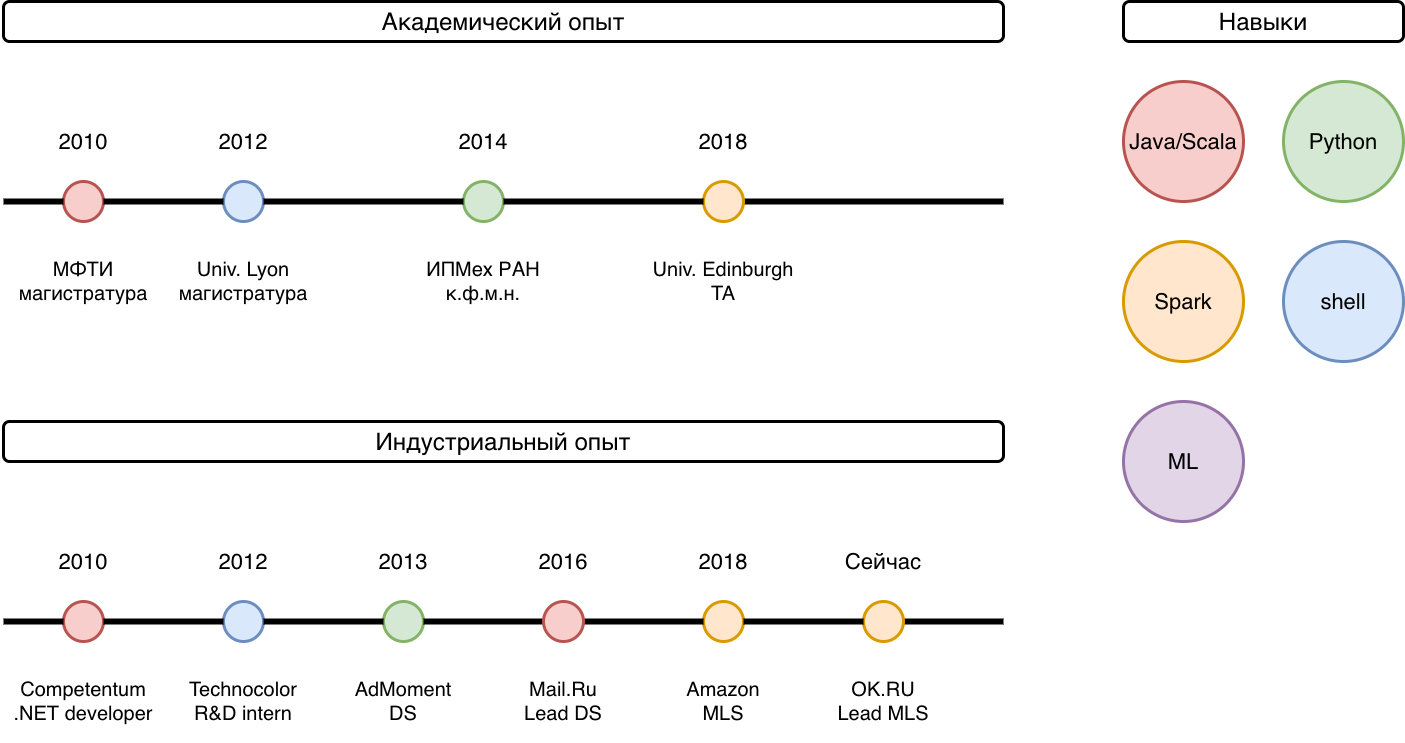
\includegraphics[scale=0.23]{images/about-me.png}
\end{center}

\end{frame}

\begin{frame}{Дарья Никанорова}

\begin{center}
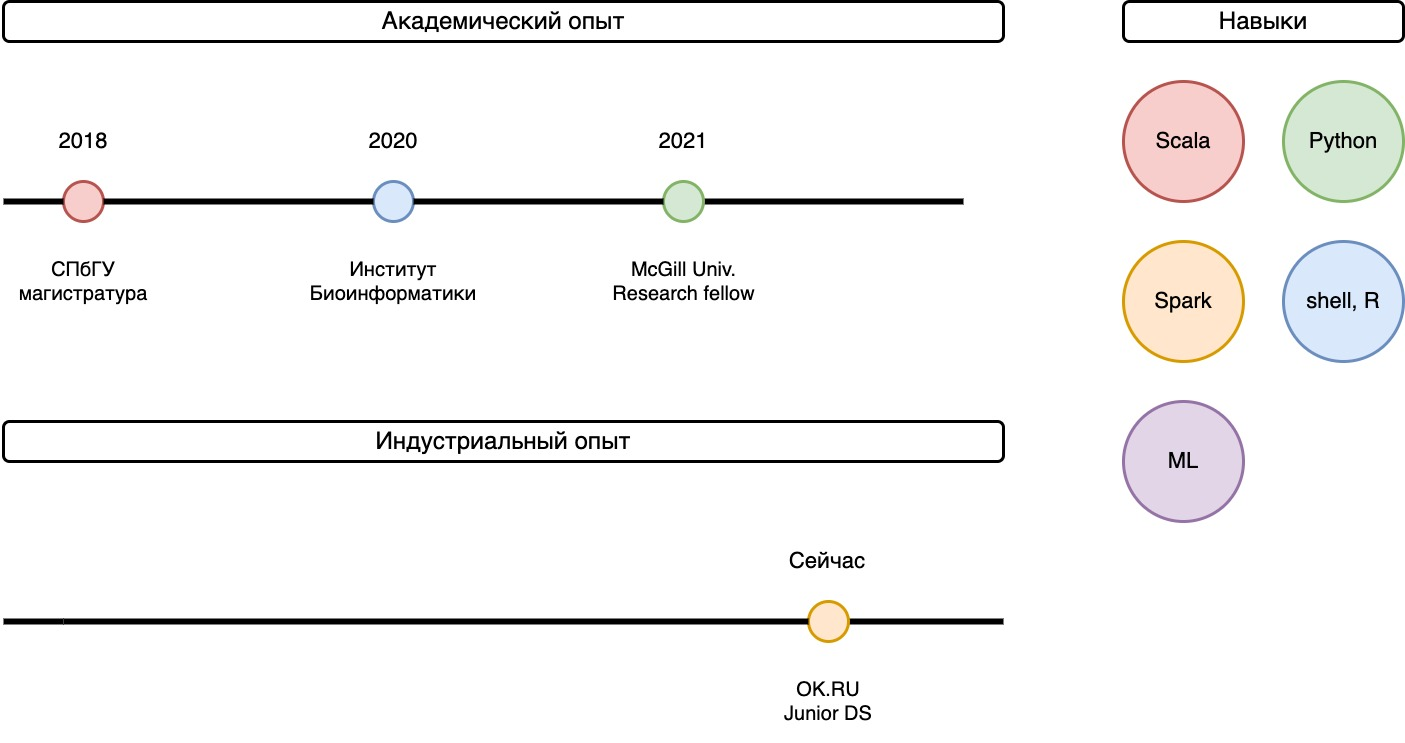
\includegraphics[scale=0.23]{images/about-me-dasha.jpg}
\end{center}

\end{frame}

\begin{frame}{Telegram}

Чат курса: \url{https://t.me/+qri5NHAS4Pc3YTky}

\vfill

\begin{itemize}
\item Вопросы вне занятия можно задать в личке или в чате курса (лучше)
\item Тегайте нас, чтобы мы не пропустили ваш комментарий в общем потоке сообщений
\item Если ответа не последовало в течении 24 часов, то мы, вероятно, не увидели ваше сообщение. Не стесняйтесь его продублировать
\end{itemize}

\end{frame}

\begin{frame}{Как задать вопрос}

\begin{itemize}
\item Голосом
\item В специально выделенное для этого время
\item Перед тем как спросить будет хорошим тоном поставить несколько знаков вопроса
\begin{tcolorbox}[colback=gray!5,colframe=gray!80,title=]
20:23 Саша: ???? \\
20:23 Преподаватель: Ждём вопроса от Саши \\
20:24 Саша: Какая метрика хорошо работает в задаче рекомендаций?
\end{tcolorbox}
\end{itemize}

\end{frame}

\begin{frame}{Если что-то пошло не так}

\begin{itemize}
\item Пропал голос
\item Исчезло изображение
\item Плохо слышно
\item Любые проблемы другого характера
\end{itemize}
\vfill
{\bf Сразу пишем в чат} много минусов и не ждем других участников. Если вы увидели, что в чате кто-то написал много минусов, а у вас всё хорошо, то поставьте несколько плюсов:
\vfill
\begin{tcolorbox}[colback=gray!5,colframe=gray!80,title=]
20:24 Петя: - - - - - - -  \\
20:25 Саша: ++++ \\
20:25 Ольга: +++++++
\end{tcolorbox}

\end{frame}

\section{Зачем нужны рекомендательные сервисы}

\begin{frame}{}

\vfill
\begin{tcolorbox}[colback=info!5,colframe=info!80,title=]
{\bf Recommender Systems} (RS) are software tools and techniques providing suggestions for {\bf items} to be of use to a {\bf user} \cite{RSHB}.
\end{tcolorbox}
\vfill
\begin{center}
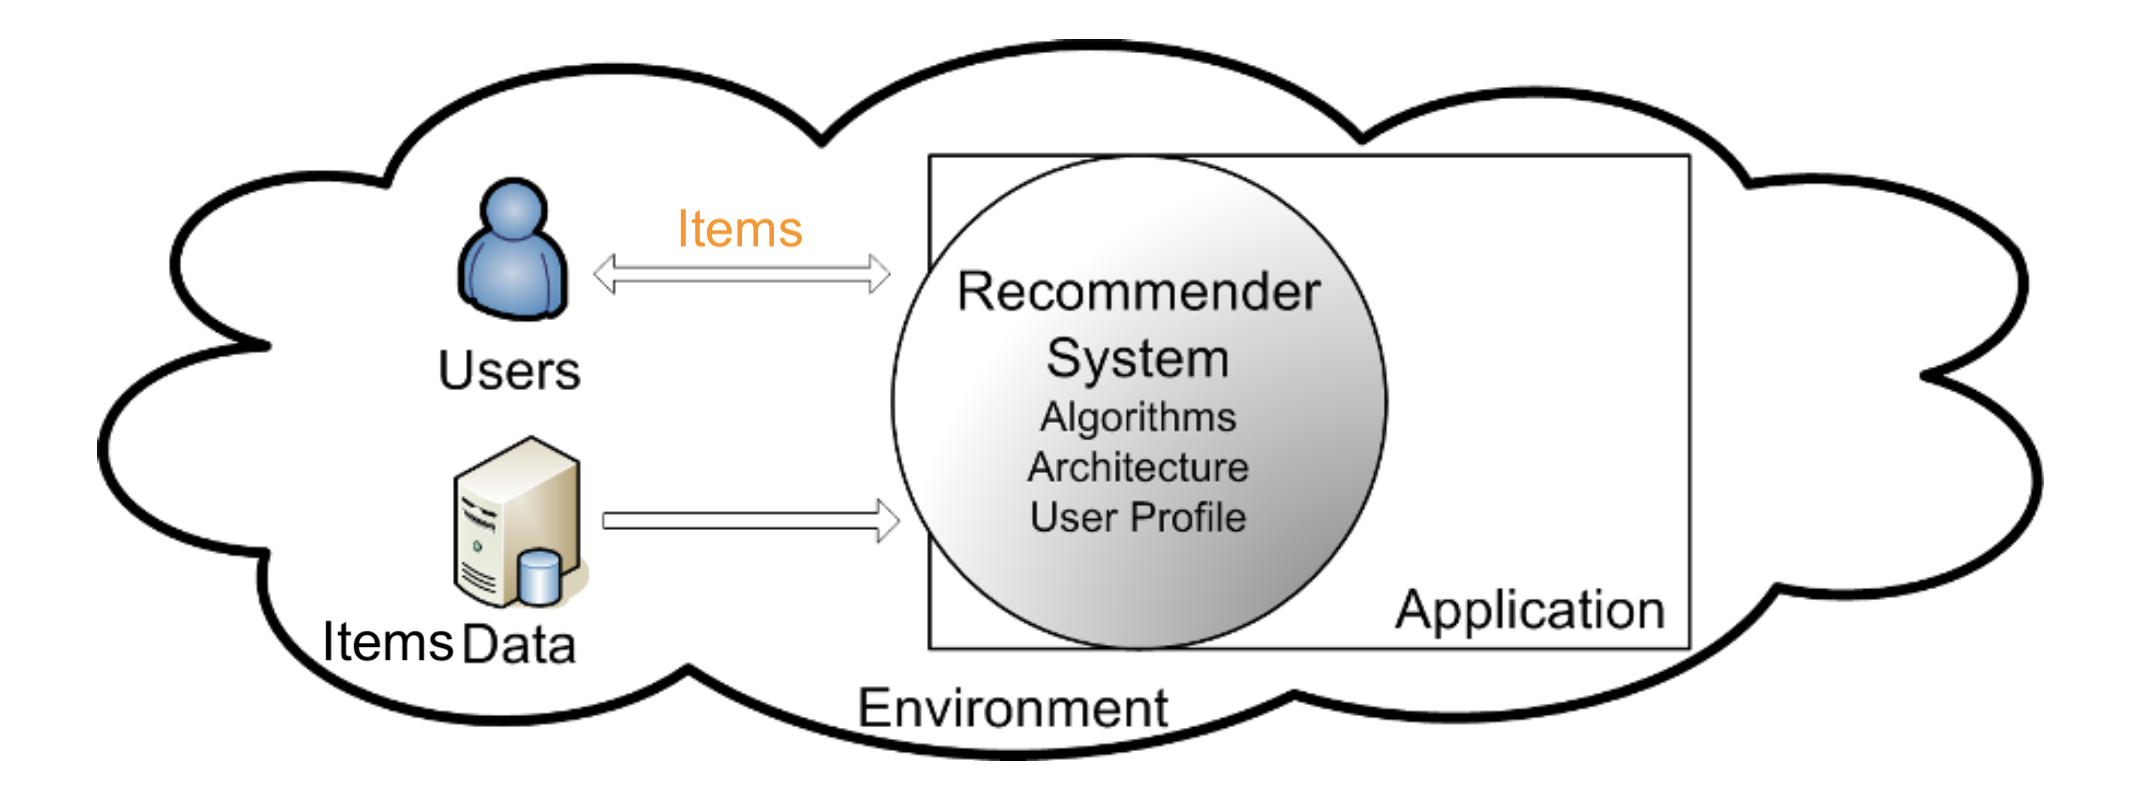
\includegraphics[scale=0.3]{images/overall.png}
\end{center}

\end{frame}

\begin{frame}{}

\begin{center}
\includegraphics[scale=0.25]{images/netflix-0.png}
\end{center}

\end{frame}

\begin{frame}{}

\begin{center}
\includegraphics[scale=0.25]{images/netflix-1.png}
\end{center}

\end{frame}

\begin{frame}{}

\begin{center}
\includegraphics[scale=0.25]{images/netflix-2.png}
\end{center}

\end{frame}

\begin{frame}{}

\begin{center}
\includegraphics[scale=0.25]{images/netflix-3.png}
\end{center}

\end{frame}

\begin{frame}{}

\begin{center}
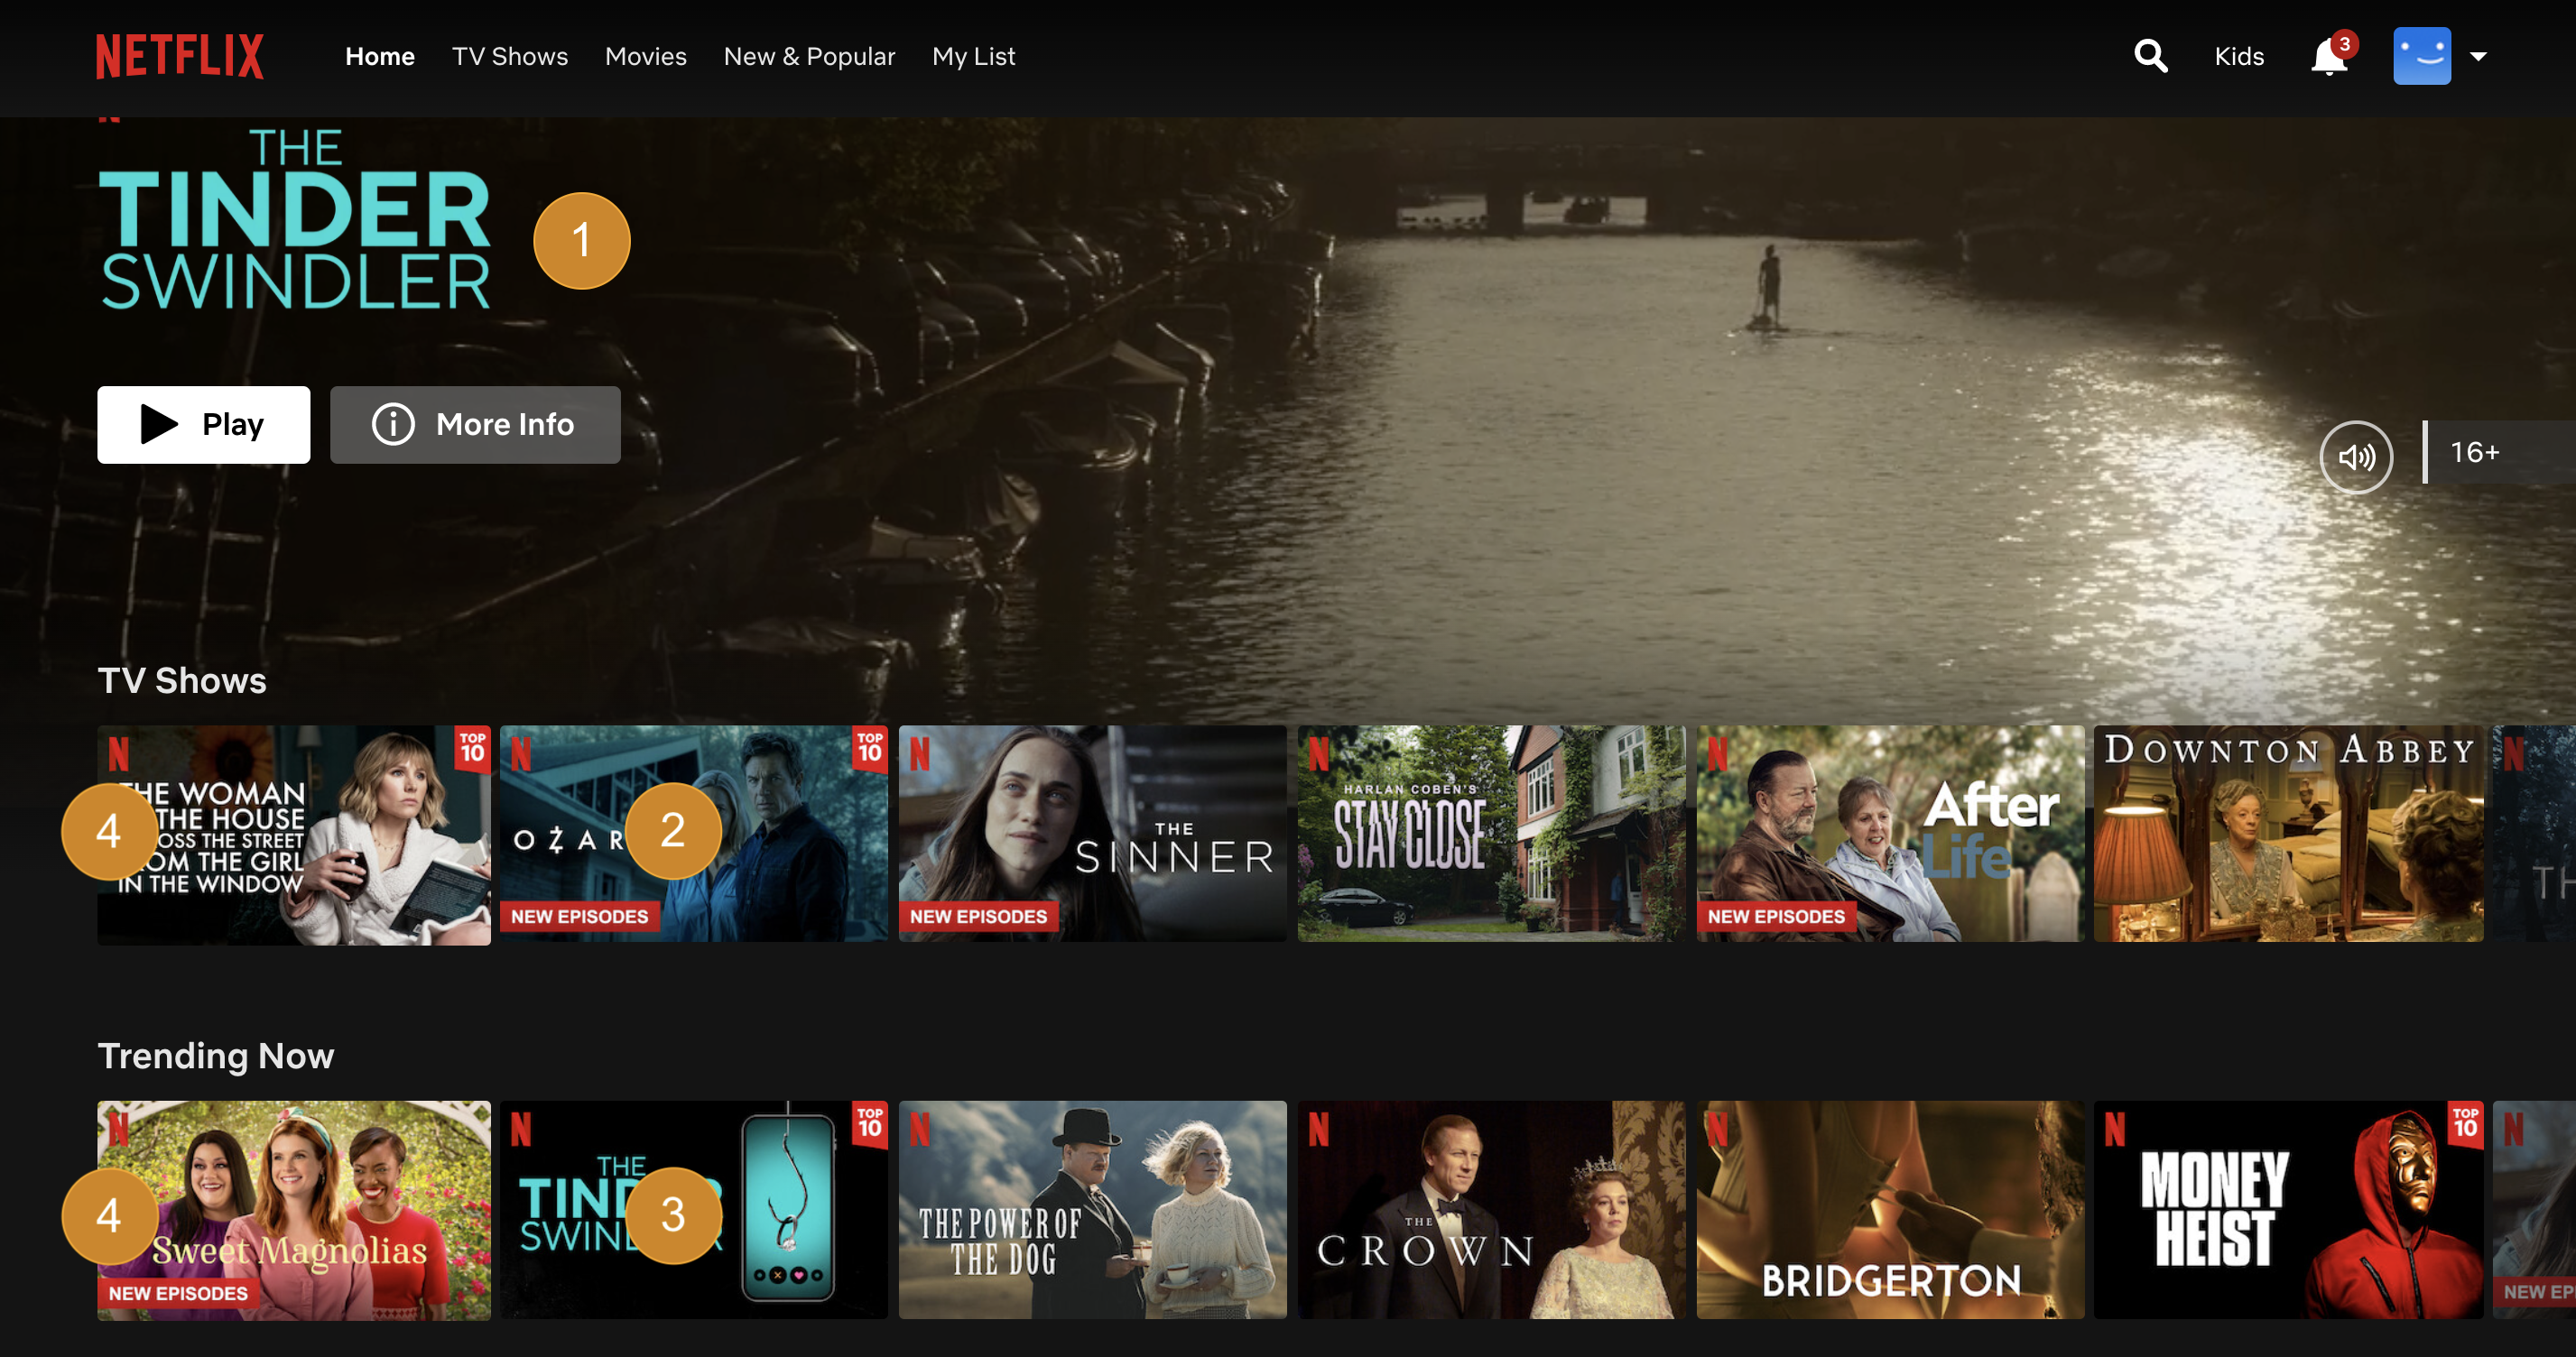
\includegraphics[scale=0.25]{images/netflix-4.png}
\end{center}

\end{frame}

\begin{frame}{}

\begin{center}
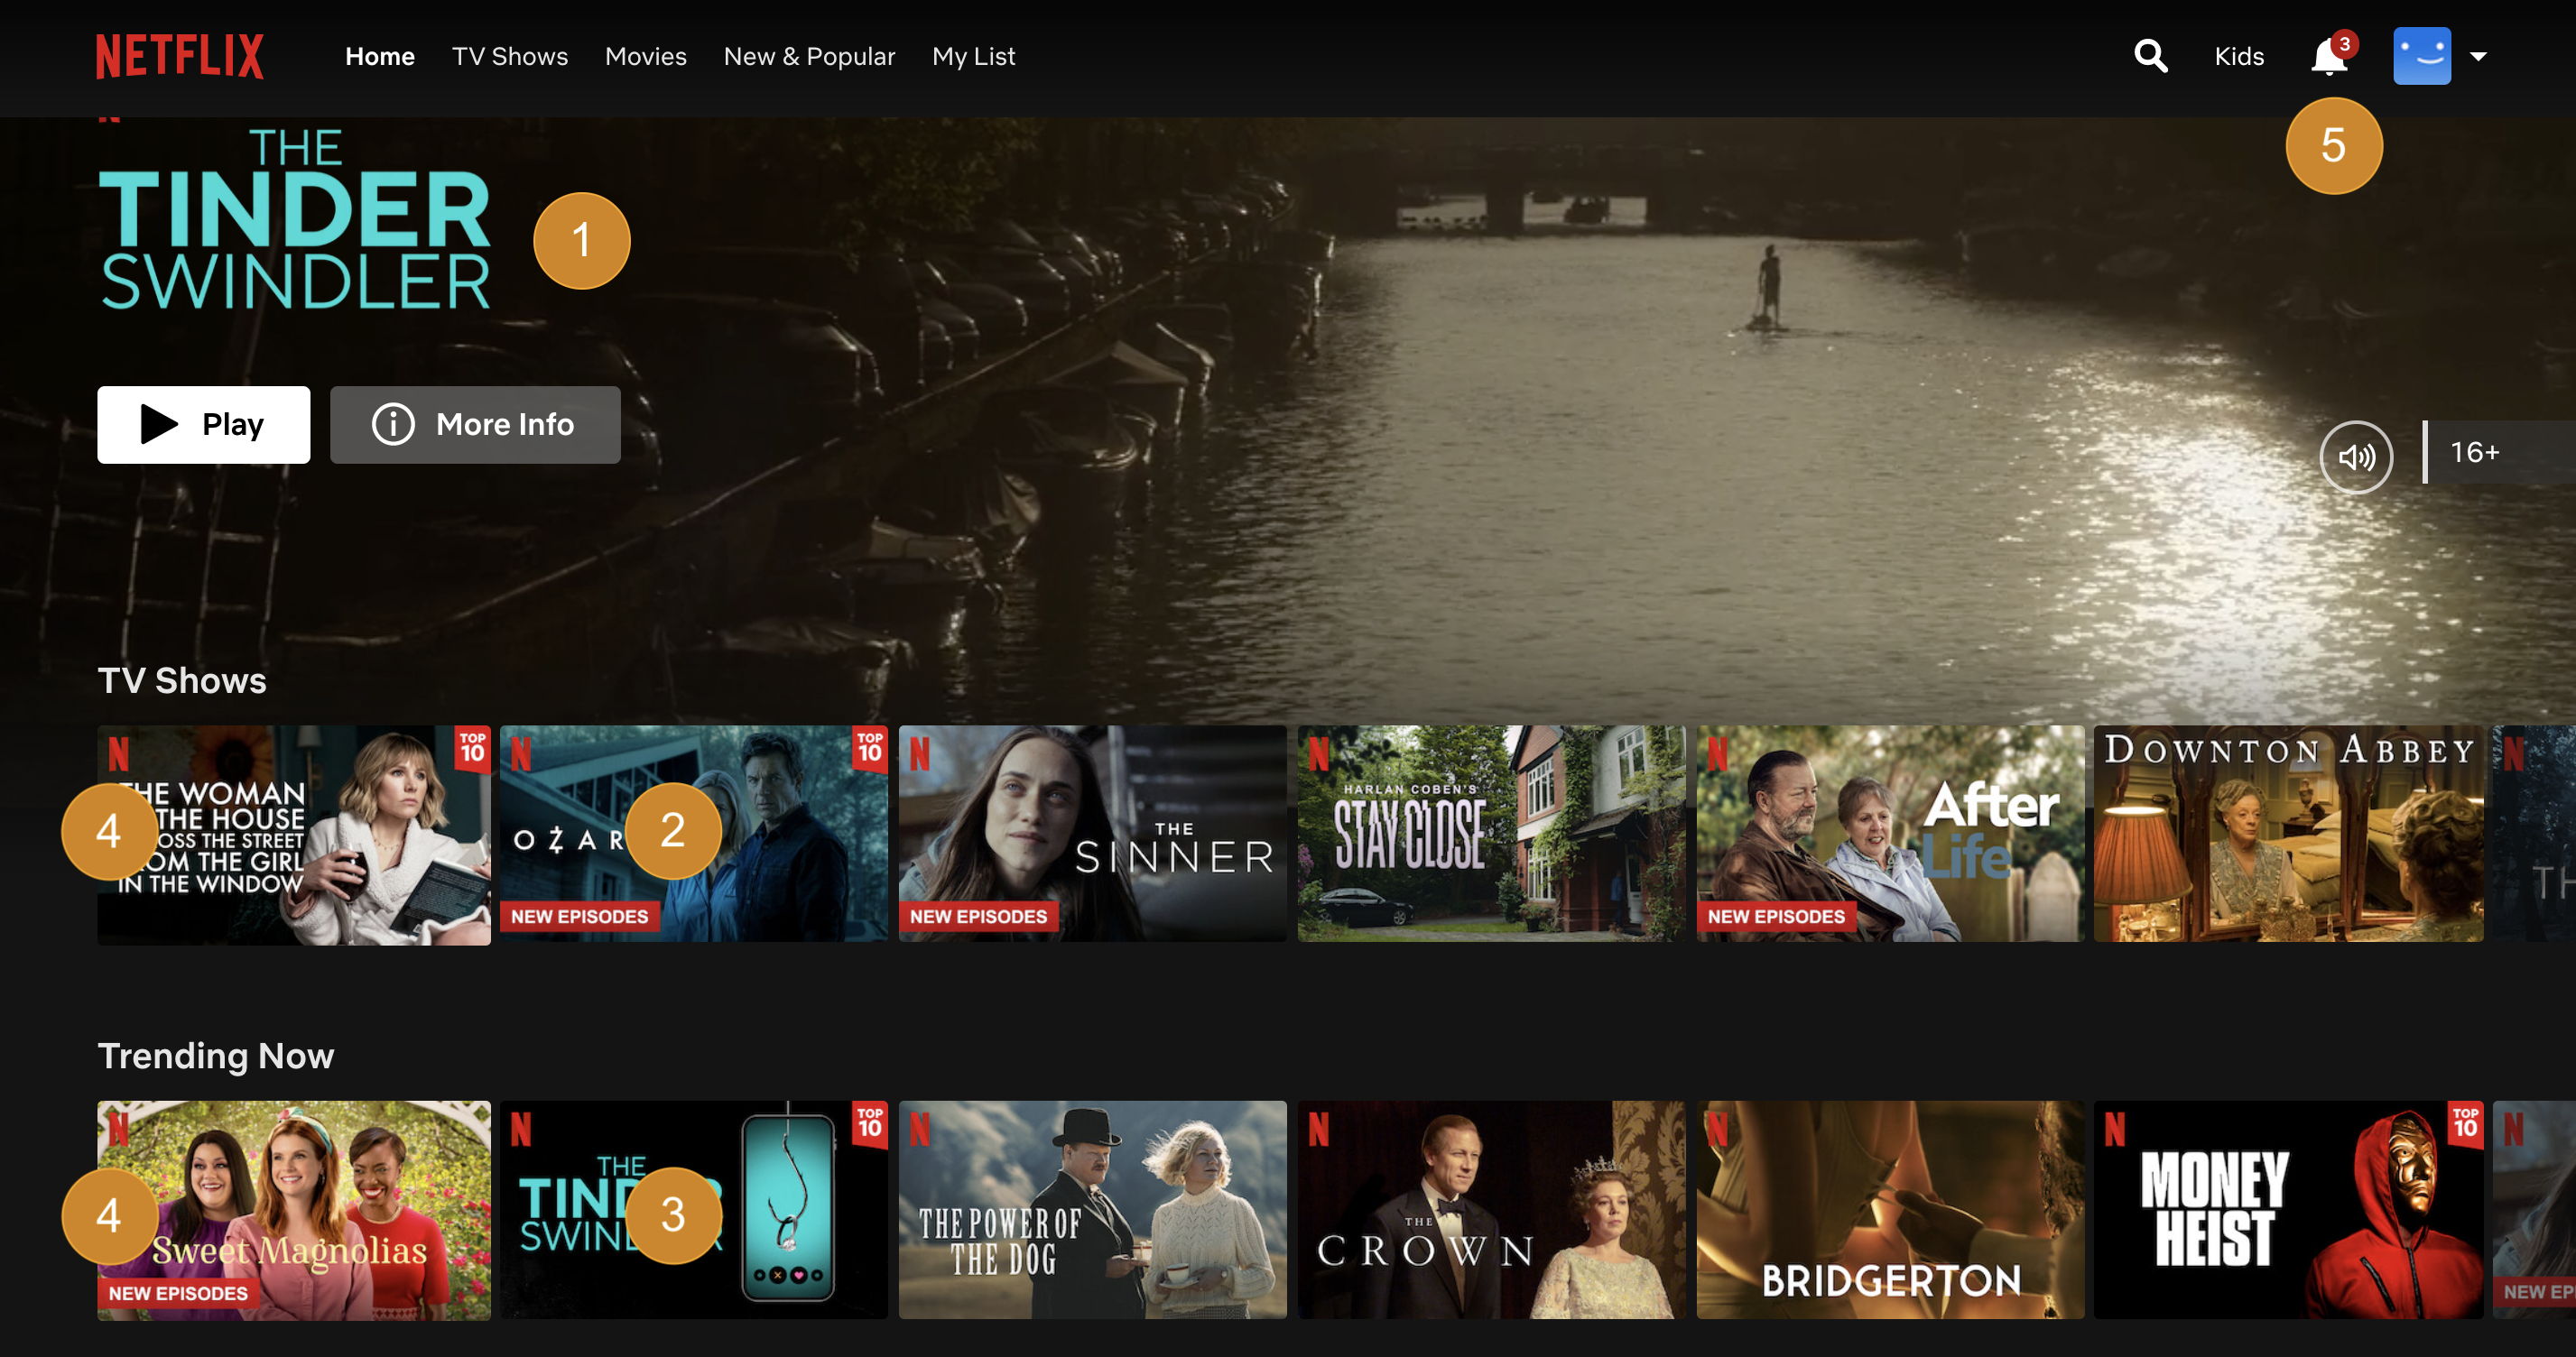
\includegraphics[scale=0.25]{images/netflix-5.png}
\end{center}

\end{frame}

\begin{frame}{}

\begin{center}
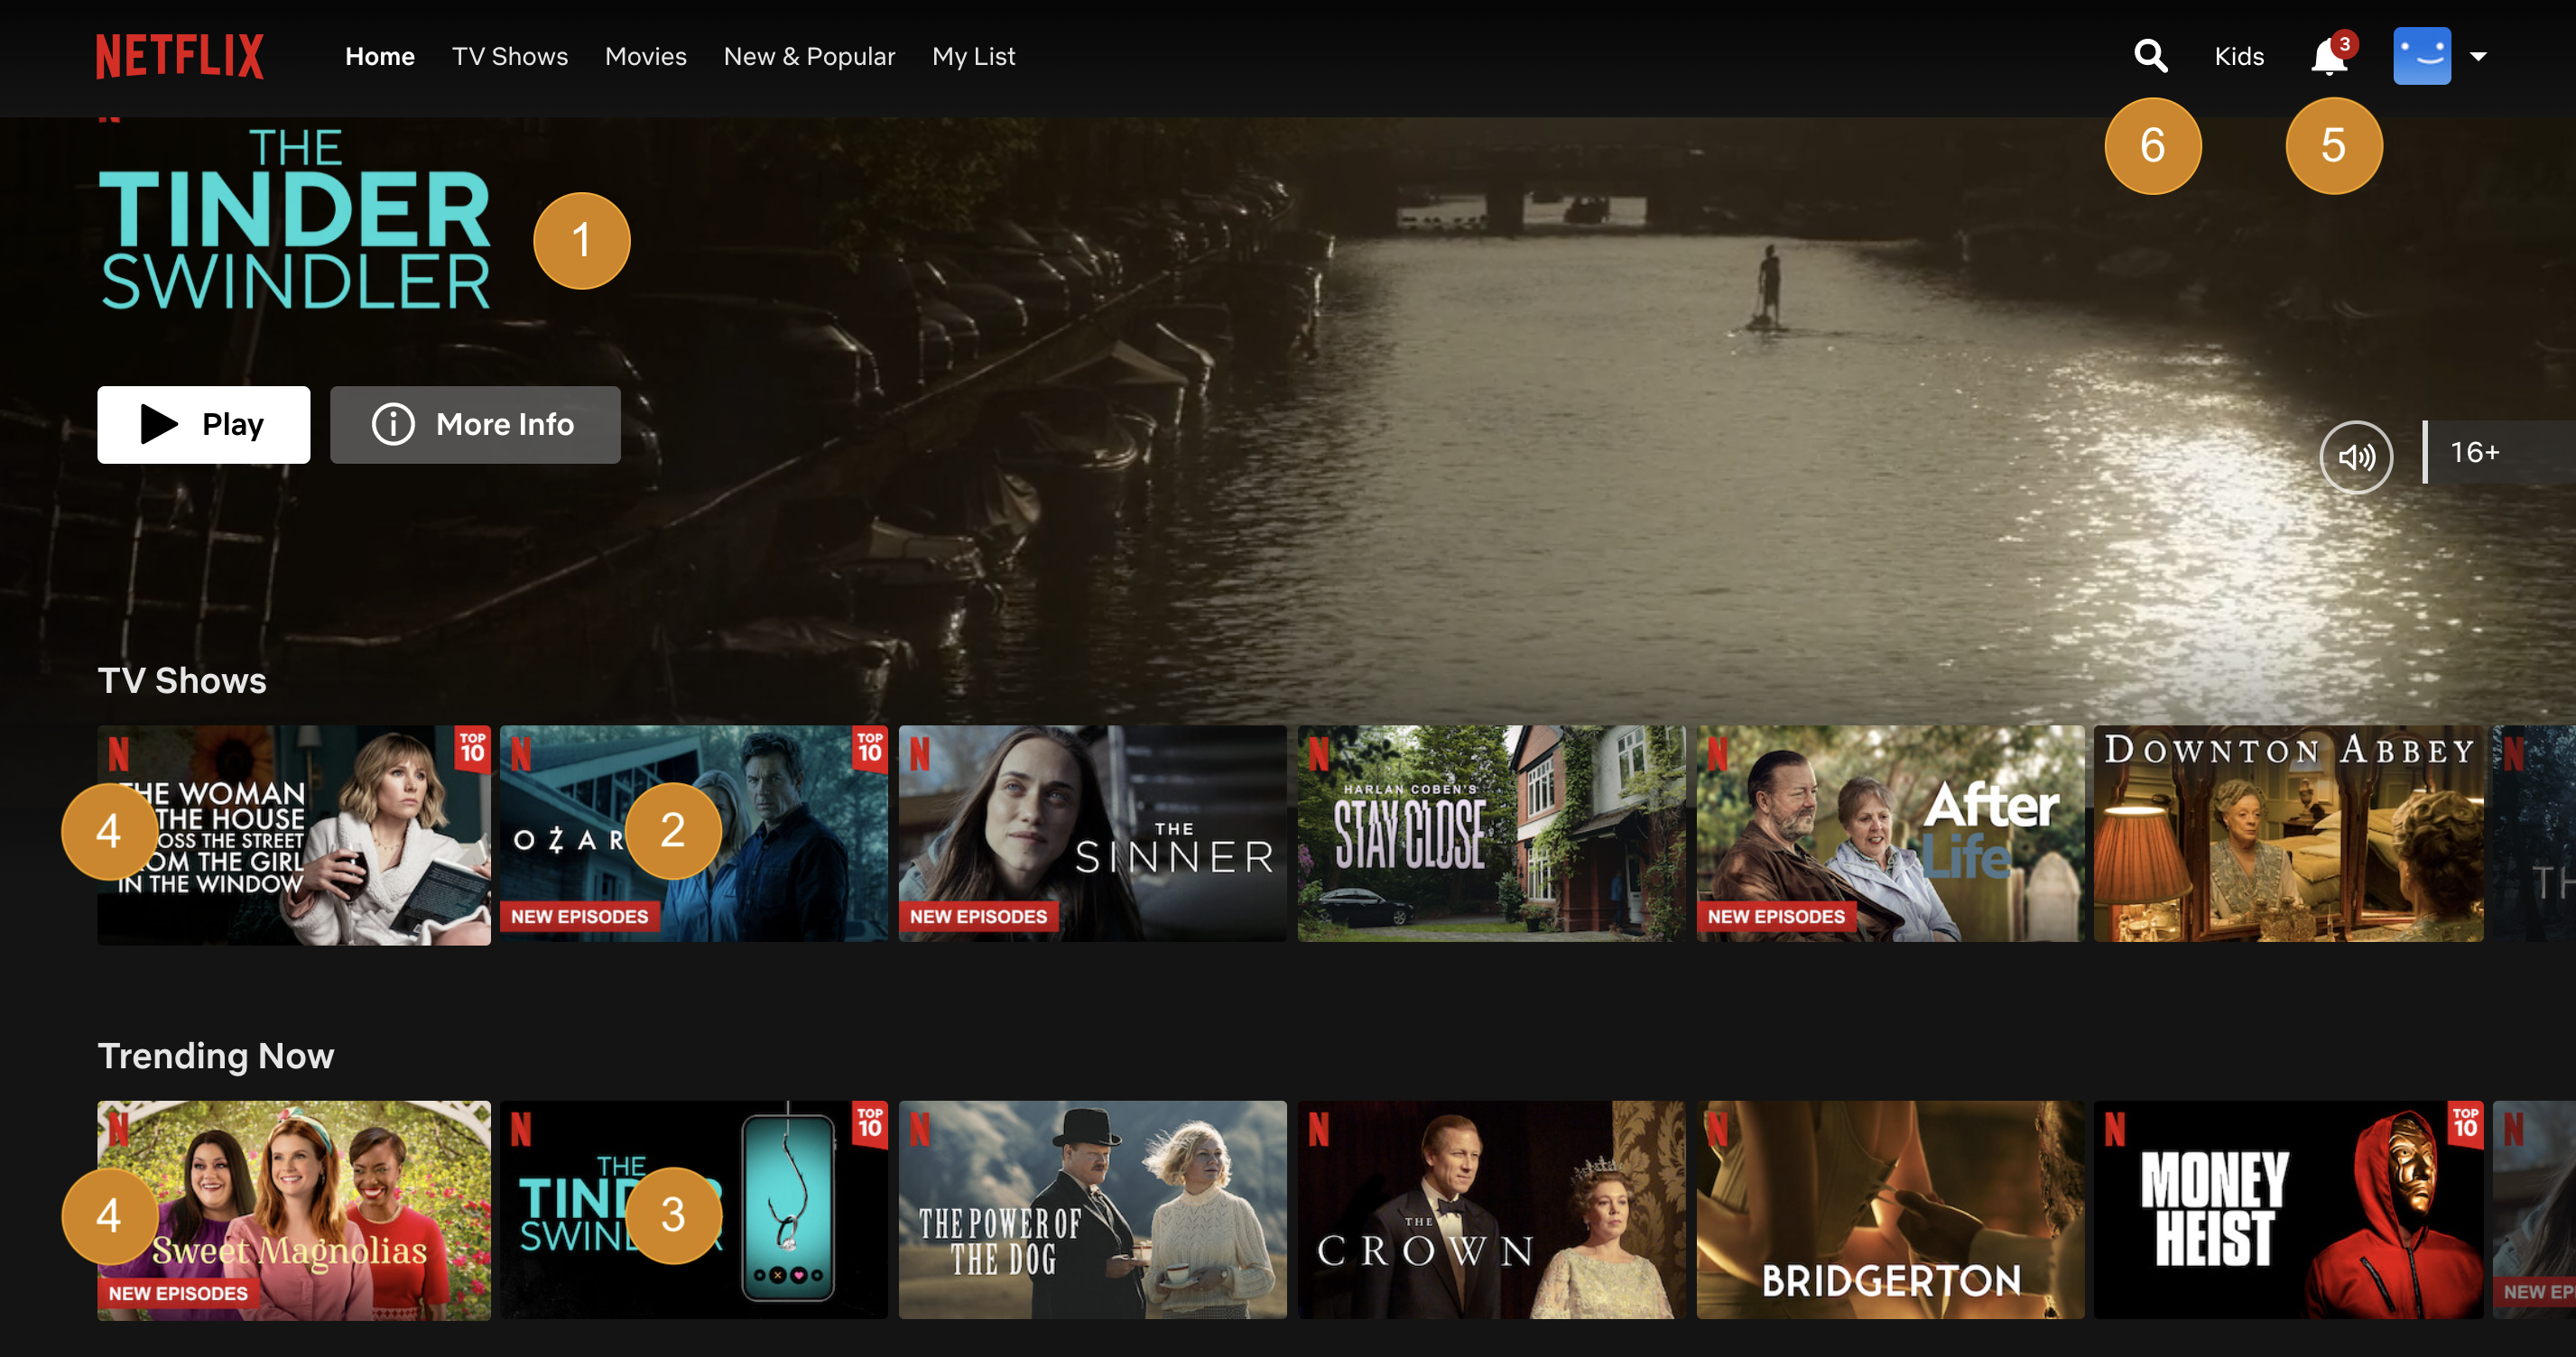
\includegraphics[scale=0.25]{images/netflix-6.png}
\end{center}

\end{frame}

\begin{frame}{RS в индустрии и науке}

{\bf Компании}

Amazon.com, YouTube, Netflix, Yahoo, Tripadvisor, Spotify, Booking.com

\vfill

{\bf Конференции}

RecSys, KDD, WSDM, SIGIR

\vfill

{\bf Книги}

Recommender Systems Handbook \cite{RSHB}, Mining of Massive datasets \cite{MMDS}

\end{frame}

\begin{frame}{Зачем RS бизнесу}

\begin{itemize}[<+->]
\item Увеличить продажи
\item Продвигать более разнообразные айтемы
\item Улучшить пользовательский опыт
\item Добиться большей лояльности
\item Лучше понимать пользователей
\end{itemize}

\end{frame}

\begin{frame}{Зачем RS пользователям}

\begin{itemize}[<+->]
\item Найти лучший айтем
\item Найти {\bf все} подходящие айтемы
\item Найти последовательность или набор айтемов
\item Залипнуть
\item Помочь другим сделать выбор
\end{itemize}

\end{frame}

\begin{frame}{Зачем RS инженерам}

\begin{columns}
\begin{column}{0.4\textwidth}
   \begin{center}
                
\includegraphics[scale=0.25]{images/computerdog.jpeg}
   \end{center}
\end{column}
\begin{column}{0.5\textwidth}
    \begin{small}
    \begin{itemize}
    \item Делать высоконагруженный отказоустойчивый сервис :D
    \item Анализировать большие данные
    \item Окунуться в волшебный мир \sout{матана} машинного обучения
    \item Объективно измерять результат своей работы 
    \item Узнать много нового о людях
    \item Все это за зарплату
    \end{itemize}
    \end{small}
\end{column}
\end{columns}

\end{frame}

\begin{frame}{RS vs другие задачи ML \cite{NETFLIX}}

\begin{itemize}[<+->]
\item RS ориентированы на продакшен
\item Наблюдаемые данные очень разреженные
\item Отсутствующие данные -- missing not-at-random
\item Отсутствующие данные -- либо ненаблюдаемые позитивные, либо негативные
\item Рекомендательные сервисы живут в петле обратной связи
\end{itemize}

\end{frame}

\begin{frame}{Пройдя этот курс, вы...}

\begin{itemize}
\item Разработаете свой рекомендательный сервис (почти) с нуля
\item Научитесь использовать Spark для нужд RS
\item Сможете выбирать правильные инструменты под конкретную задачу
\item Узнаете о проблемах, возникающих в боевых RS, и научитесь их решать
\item Будете в курсе SOTA моделей и задач RS, над которыми работают ученые
\item Подготовитесь к собеседованию по RS на junior позицию
\end{itemize}

\end{frame}

\section{Что дальше}

\begin{frame}{Программа модуля}
\begin{small}
\begin{tabular}{ c | l | c | c | c }
{\bf Неделя} & {\bf Тема} & {\bf Квиз} & {\bf Семинар} & {\bf Домашка} \\
\hline
1 & Рекомендательные сервисы в продакшене & \checked  & \checked &  \\
2 & Метрики и базовые подходы & \checked  &  \checked &  \\ 
3 & Классические алгоритмы 1 & \checked  & \checked & \\
4 & Классические алгоритмы 2 & \checked  & \checked & \checked  \\
5 & Нейросетевые рекомендеры & \checked  & \checked &  \\
6 & Нерешенные проблемы и новые направления & \checked  &  \checked & \\
7 & Рекомендации и Reinforcement Learning & \checked  & \checked & 
\end{tabular}
\end{small}
\end{frame}

\begin{frame}{Оценка $\in [0, 1]$}

\begin{itemize}
\item Идеальное выполнение домашки = 0.6 (нижняя граница ``тройки'')
\item Идеальное выполнение квизов и домашки = 0.9 (нижняя граница ``пятерки'')
\item Выберем трех самых активных слушателей и накинем им по 0.1
\item Дополнительные баллы можно получить на зачете
\end{itemize}

\end{frame}

\begin{frame}{}

\begin{center}

\includegraphics[scale=1.0]{images/welcome.jpeg}
\end{center}

\end{frame}

\begin{frame}[allowframebreaks]{Литература}
\bibliographystyle{amsalpha}
\bibliography{references.bib}
\end{frame}

\end{document}
